\documentclass[brazil,hardcopy,openany,a4paper]{ufscthesis}
\usepackage[brazil]{babel}
\usepackage{amsfonts, amsmath, amsthm, amsbsy,amssymb,bm,mathtools} % For math fonts, symbols and environments %
\usepackage{graphicx} 		% Required for including images
\usepackage{transparent}	% may be required for inkscape pdf figures (http://bit.ly/18i5Oga)
\usepackage{listings}
\usepackage{caption}
\usepackage{multirow}
\usepackage{lscape}
\usepackage[T1]{fontenc}
\sloppy
\usepackage{siunitx}
\usepackage{nameref}
\usepackage{float}

\newcommand{\source}[1]{\small \caption*{Fonte: {#1}} } % Criar fonte embaixo da figura

\newsubfloat{figure}		% Allow subfloats in figure environment (http://bit.ly/1C20NAj)
\graphicspath{{figures/}} 	% Location of the graphics files

\usepackage{siunitx} % units package
\let\DeclareUSUnit\DeclareSIUnit
\let\US\SI
\let\us\si
\DeclareUSUnit\inch{in}
\sisetup{detect-all}  %it may be necessary to load it after loading the font package


%----------------------------------------------------------------------
% Comandos criados pelo usuário
\newcommand{\afazer}[1]{{\color{red}{#1}}} % Para destacar uma parte a ser trabalhada
\DeclareMathOperator*{\argmin}{\arg\!\min}
\DeclareMathOperator*{\argmax}{\arg\!\max}

%----------------------------------------------------------------------
% Identificadores do trabalho
% Usados para preencher os elementos pré-textuais
\instituicao[a]{Universidade Federal de Santa Catarina} % Opcional
\departamento[a]{Biblioteca Universitária}
\programa[o]{Programa de Pós-Graduação em Engenharia Civil} 
\curso{Engenharia de Engenharia Civil}
\documento[a]{Dissertação} % [o] para dissertação e trabalho de conclusão de curso [a] para tese
\grau{Mestre} % doutor, mestre, engenheiro, etc.
\titulo{Modelagem do impacto da ilha de calor sobre o desempenho energético de escritórios condicionados artificialmente}
\subtitulo{} % Opcional
\autor{Marcelo Salles Olinger}
\local{Florianópolis} % Opcional (Florianópolis é o padrão)
\data{24}{junho}{2019}
\orientador[Universidade Federal de Santa Catarina]{Profa. Ana Paula Melo, Dra.}
\coordenador[Universidade Federal de Santa Catariana]{Prof. Fulano de Tal, Dr.}
\orientadornabanca{sim} % Se faz parte da banca definir como sim
\coorientadornabanca{nao} % Se faz parte da banca definir como sim
\bancaMembroA{Prof. Saulo Guths, Dr.\\Universidade Federal de Santa Catarina}  %Nome do presidente da banca
\bancaMembroB{Prof. Membro Dois, Dr.\\Universidade Federal de Santa Catarina}   % Nome do membro da Banca
\bancaMembroC{Profa. Membro Três, Dra.\\Outra Universidade} % Nome do membro da Banca
% \bancaMembroD{Quarto membro\\Universidade ...} % Nome do membro da Banca
% \bancaMembroE{Quinto membro\\Universidade ...}  % Nome do membro da Banca
% \bancaMembroF{Sexto membro\\Universidade ...}   % Nome do membro da Banca
% \bancaMembroG{Sétimo membro\\Universidade ...}  % Nome do membro da Banca

%\dedicatoria{Dedico essa conquista aos amigos e familiares que tornaram isso possível.}

%\agradecimento{Inserir os agradecimentos aos colaboradores à execução do trabalho. Inserir os agradecimentos aos colaboradores à execução do trabalho.}

%\epigrafe{Se você pensa que pode ou se pensa que não pode, de qualquer forma você está certo.}{Henry Ford}

\textoresumo {}
\palavraschave{Ventilação natural. Metamodelo. Simulação termoenergética de edificações.}

\textabstract {Text...}
\keywords{Word 1. Word 2. Word 3.}

\begin{document}
	\mainmatter

\chapter{Revisão de literatura}
	
	\section{Ventilação natural}
	
	A ventilação natural (VN) ocorre quando diferenças de pressão geradas pelo vento ou por forças de empuxo agem em uma ou mais aberturas da envoltória de uma edificação \cite{CarrilhodaGraca2016}. Um sistema de VN pode ser caracterizado pela estratégia de ventilação, locação das aberturas e suas áreas.  \citeonline{CarrilhodaGraca2016} comentam que, apesar de muitos regulamentos exigirem uma área mínima de ventilação, tipicamente definida em função da área de piso, essas exigências se baseiam em grandes simplificações. A área de abertura ideal depende da estratégia de ventilação (unilateral ou cruzada), do clima e dos objetivos relacionados ao período de uso da VN.
	
	A VN pode ser aplicada por meio de grelhas, sistemas de dutos, ou simplesmente grandes aberturas, como janelas ou portas. No caso de grandes aberturas, duas configurações podem ser consideradas: ventilação cruzada, ou ventilação unilateral. Na estratégia ventilação unilateral, a turbulência do vento e as variações nos gradientes de pressão induzidos por rajadas podem afetar fortemente o fluxo de ar nas aberturas.
	Como esses parâmetros não são estáveis, é mais complicado avaliar a ventilação unilateral em relação à ventilação cruzada \cite{Freire2013}.
	\citeonline{CarrilhodaGraca2016} apontam que para otimização da VN unilateral em edificações pequenas ou médias, para a mesma área total de abertura, duas ou mais aberturas são mais eficientes do que apenas uma, sendo que aberturas espaçadas funcionam melhor do que próximas.	% Ver Stabat, P., Caciolo, M., & Marchio, D. (2012). Progress on single-sided ventilation techniques for buildings. Advances in Building Energy Research, 6(2), 212–241. https://doi.org/10.1080/17512549.2012.740903
	Além das diferentes estratégias relacionadas à configuração das aberturas na edificação, há também diferentes abordagens quanto aos períodos de funcionamento. Algumas edificações podem permitir o uso da VN durante o dia, enquanto outras também permitem o uso de VN noturna. Há também casos em que a VN é exclusivamente noturna, e durante o dia utiliza-se sistemas de condicionamento de ar \cite{Pesic2018}.
	
	O mecanismo de ventilação natural noturna é baseado na transferência de calor por convecção da estrutura exposta do edifício para o fluxo de ar frio da noite (momento em que a diferença entre a temperatura do ar interno e externo é maior) \cite{Breesch2010}. Durante o dia, a massa térmica da	edificação é utilizada para acumular os ganhos de calor internos e do sol, e prevenir condições desconfortáveis durante as horas de operação da edificação.	
	Isso leva a três consequências: para garantir o funcionamento, o calor deve ser armazenado na estrutura da edificação, e é necessário garantir uma ponte para que haja a transferência de calor para/da estrutura; a ventilação noturna é mais apropriada para climas moderados e frios, com maiores diferenças diárias de temperatura ao longo do dia; como essa tecnologia utiliza apenas calor sensível, é menos aplicável em climas quentes e úmidos.
	
	Prover, efetivamente, VN em edifícios pode economizar energia e custo em comparação à ventilação mecânica devido à baixa manutenção e custo zero de operação \cite{Omrani2017}. O desempenho da VN é medido, primariamente, através de parâmetros de dinâmica dos fluidos, como padrão do fluxo de ar, velocidade média, taxa de fluxo de ar, distribuição de pressão, renovações de ar, fluxo volumétrico e outras qualidades que podem ser derivadas desses parâmetros.
	Esses elementos do fluxo também podem ser usados para determinar características mais amplas do ambiente interno de edificações, como a qualidade do ar e o conforto térmico. Há diferentes métodos de avaliação de desempenho de VN, cada um com suas vantagens e limitações. O método escolhido deve ser o mais apropriado, baseado nos recursos, exigências e estágio do projeto.
	
	Estimar o desempenho da VN no projeto da edificação envolve a consideração de fenômenos físicos complexos, o que pode ser dificultoso. Para a simulação computacional, há duas principais formas de descrever a ventilação natural: \textit{Computer Fluid Dynamics} (CFD) e \textit{Airflow Network} (AFN). O CFD utiliza equações de Navier-Stokes para resolver diretamente o problema do fluxo de ar através das propriedades da dinâmica dos fluidos \cite{Arendt2017}. Apesar do grande custo computacional, o CFD disponibiliza informações detalhadas sobre a distribuição da velocidade do ar, temperatura, pressão e concentração de partículas na área analisada. No entanto, bons resultados com o uso dessa ferramenta dependem da qualidade da grade adotada, da aplicação correta das condições de contorno, e da aplicação correta das diversas suposições tomadas ao adotar-se modelo. 
	
	O AFN funciona a partir de uma rede de nós, análoga a um circuito elétrico. A cada zona térmica da edificação é atribuído um nó, e os caminhos do fluxo recebem uma resistência equivalente para cada ligação entre as zonas.
	Condições dentro da zona, como velocidade do ar, temperatura, umidade são então computadas com base nas diferenças de pressão entre as zonas definidas e são comumente resolvidas em condições estacionárias \cite{Omrani2017}.	
	O uso de modelos multi-zona exige a suposição de que o ar dentro de cada zona é homogêneo, com temperatura, velocidade, concentração de contaminantes e umidade relativa uniformes. Modelos multi-zona são úteis na predição do desempenho de VN do edifício, por prover resultados robustos. Porém, não podem prover informações detalhadas sobre o comportamento do ar dentro da zona. Apesar de ser uma abordagem muito mais simplificada, o AFN é muito utilizado em razão da facilidade de aplicação e por ter um custo computacional muito mais baixo, quando comparado ao CFD. Ferramentas de simulação computacional, como o programa EnergyPlus, podem integrar o modelo térmico de um edifício com um modelo AFN \cite{Belleri2014}.
	
	O modelo de pressão e fluxo de ar utilizado pelo EnergyPlus \cite{EnergyPlus2018} foi desenvolvido baseado no modelo AIRNET \cite{Walton1989}. Os cálculos de fluxo de ar multi-zona são realizados no timestep do sistema HVAC (\textit{Heating, Ventilation and Air-Conditioning}). O modelo de rede de fluxo de ar consiste em três passos sequenciais:
	
	1- cálculos de pressão e fluxo de ar;
	
	2- cálculos de temperatura e umidade no nó;
	
	3- cálculos de carga sensível e latente.
	
	Os cálculos de pressão e fluxo de ar determinam, a partir das pressões de vento e fluxos de ar forçados, a pressão em cada nó e o fluxo de ar através de cada ligação. Baseando-se no fluxo de ar calculado para cada ligação, o modelo	calcula as temperaturas e umidades relativas em cada nó a partir das temperaturas e umidades relativas das zonas. 
	Utilizando as temperaturas e umidades relativas calculadas, as cargas latentes e sensíveis conduzidas pelos	sistemas de fluxo forçado e das infiltrações são somadas em cada zona. As cargas latentes e sensíveis obtidas nessa etapa são utilizadas então nas equações de balanço energético das zonas para predizer possíveis cargas relacionadas ao sistema HVAC e calcular as temperaturas do ar, umidades relativas e pressões finais da zona.
	
	Uma ligação utilizada no modelo do AFN tem dois nós, um de entrada e um de saída, e possui um componente que determina a relação entre o fluxo de ar e a pressão. A diferença de pressão entre cada componente em uma ligação é calculada pela equação de Bernoulli \cite{Walton1989}. Como apresentado na Figura \ref{fig:nos_AFN}, cada nó é atribuído a uma zona e cada ligação corresponde a um elemento de resistência entre os nós, que pode representar uma abertura, ou uma superfície com frestas.
	
	\begin{figure}[]
		\centering
		\caption{Relação entre nós e ligações do AFN.}
		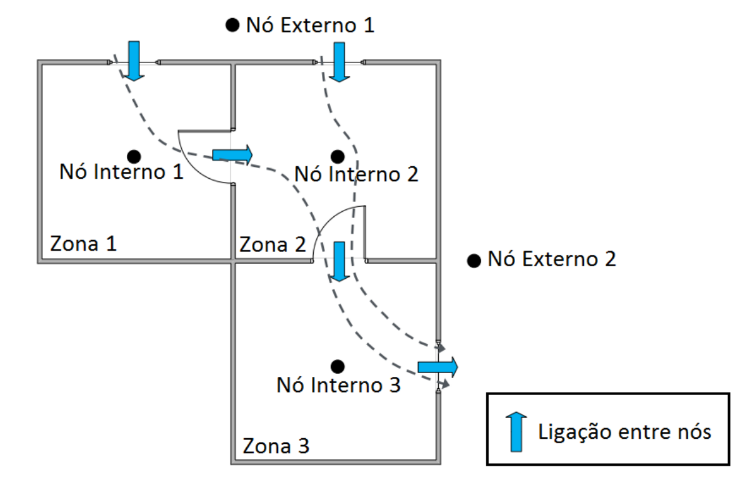
\includegraphics[width=1\linewidth]{img/nos_AFN.png}
		\label{fig:nos_AFN}
			\begin{flushleft}
				Fonte: adaptado de \citeonline{EnergyPlus2018}.
			\end{flushleft}
	\end{figure}
	
	A velocidade na qual se considera que o vento atinge a edificação modelada é obtida a partir do arquivo climático utilizado na simulação computacional. A partir das medições de velocidade do vento na estação meteorológica, extrapola-se os valores para as outras altitudes e os perfis de terreno. Essa consideração em relação à velocidade do vento é baseada no \textit{Handbook of Fundamentals} da \citeonline{ASHRAE2005}.
	
	Os coeficientes do perfil de velocidade do vento são variáveis que dependem das características de rugosidade do terreno no entorno. Os valores típicos são apresentados na Tabela \ref{tab:ventoterreno}.
	
	\begin{table}[h]
%		\vspace{-10pt}
		\caption{Coeficientes do perfil de velocidade do vento.}
		\label{tab:ventoterreno}
		\centering
		\resizebox{\textwidth}{!}{
		\begin{tabular}{|c |c |c |c | } % \textwidth}{@{\extracolsep{\fill}} \hspace{-.33\columnwidth}
			\hline	
			\textbf{Categoria} & \textbf{Descrição do terreno} & \textbf{Expoente,} & \textbf{Espessura da camada} \\
			\textbf{do terreno} & {} & \textbf{$\alpha$} & \textbf{limite, $\delta$ (m)} \\
			\hline
			{} & Grandes centros urbanos nos quais & {} & \\
			1 & pelo menos 50\% das edificações são & 0,33 & 460 \\
			{} & maiores que 21 m. & {} & \\
			\hline
			{} & Terreno urbano, subúrbio, áreas com & {} & \\
			2 & árvores, áreas com espaçamento & 0,22 & 370 \\
			{} & entre obstruções do tamanho ou & {} & \\
			{} & maiores do que casas unifamiliares. & {} & \\
			\hline
			{} & Terreno aberto com poucas & {} & \\
			3 & obstruções, geralmente menores do & 0,14 & 270  \\
			{} & que 10 m de altura. & {} & \\
			\hline
			{} & Área desobstruída plana exposta ao & {} & \\
			4 & vento. Entorno de corpos d’água de & 0,10 & 210  \\
			{} & mais de 1,6 km. & {} & \\
			\hline
			
		\end{tabular}
	}
	\begin{flushleft}
		Fonte: adaptado de \citeonline{ASHRAE2005} (tradução do autor).
	\end{flushleft}
%		\vspace{-12pt}
	\end{table}
	
	O valor padrão para a medição da velocidade de vento é de 10 m de altitude. Os valores padrão para $\alpha_{met}$ e $\delta_{met}$ são 0,14 e 270 m, respectivamente, porque a maioria das estações meteorológicas estão localizadas em campos abertos.
	
	Ao definir a velocidade do vento, o programa EnergyPlus calcula a pressão do vento sobre as edificações, determinada também pelo princípio da equação de Bernoulli \cite{Walton1989}.
	
	A maior dificuldade no desenvolvimento do AFN é a necessidade de estimar as características do fluxo nas aberturas e o coeficiente de pressão do vento na edificação \cite{Arendt2017}. Os coeficientes de pressão do vento (Cp) descrevem como o vento interfere na distribuição externa de pressões em volta da edificação. 
	Os Cp dependem principalmente da geometria da edificação, dos detalhes da fachada, do entorno da edificação, da velocidade e direção do vento, e da intensidade da turbulência. Na prática, 	destaca-se a dificuldade em determinar precisamente a relação entre o Cp e todos esses fatores. As abordagens mais realistas são os experimentos em escala real in-situ. No entanto, esses experimentos possuem custo elevado e normalmente possuem grandes incertezas. Os dados dos Cp podem ser estimados das seguintes fontes: testes de túnel de vento; simulações com CFD; modelos analíticos; e bases de dados.
	Bases de dados de Cp são compilações de uma ou mais fontes, onde os dados são classificados de acordo com alguns parâmetros, como a forma da edificação e a orientação de incidência do vento. 
	
	A dificuldade em se considerar toda a complexidade de variação do Cp faz com que os programas de simulação termoenergética de edificações com AFN, geralmente, incorporem métodos simplificados \cite{Costola2009}. Os experimentos de túnel de vento são as fontes primárias mais comuns. A qualidade dos resultados de túneis de vento são diretamente afetados pela calibração do túnel de vento, a garantia de qualidade dos procedimentos, e o conhecimento do pessoal para a preparação e execução dos testes.
	
	Os túneis de vento permitem um bom grau de controle sobre os experimentos, assim como a repetitividade e reprodutibilidade dos testes conduzidos \cite{Omrani2017}. No entanto, a escala pode afetar o fluxo de ar e as transferências de calor se os parâmetros adimensionais corretos não são mantidos entre os modelos de diferentes tamanhos. Isso faz com que o ideal seja usar modelos em escala real.
	
	Em casos em que não é possível obter os valores de Cp por fontes primárias, \citeonline{Costola2009} apontam as bases de dados como as fontes secundárias mais comuns. A base de dados de pressão de vento da Universidade Politécnica de Tóquio (TPU) oferece dados experimentais obtidos a partir de experimentos em túnel de vento \cite{TPU2018}. A base de dados possui os resultados de testes conduzidos utilizando-se modelos de acrílico em um túnel de vento de seção de 2,2 m de largura por 1,8 m de altura. A camada limite atmosférica foi simulada por elementos geradores de turbulência e outros elementos de rugosidade. Diferentes perfis de vento foram usados para construir a base de dados. Na maioria dos experimentos a velocidade média e os perfis de intensidade de turbulência estavam de acordo com as de terreno suburbano. A intensidade de turbulência à altura de 10 cm foi cerca de 0,25, e a velocidade de vento teste a essa altura foi 7,4 m/s. O número mínimo de Reynolds foi 25340, que é acima do limite 11000 para o fluxo independente.
	
	Diversos fatores que afetam o valor do Cp são comumente simplificados, como apontado por \citeonline{Costola2010} na Tabela \ref{tab:CpSimp}.
	
	\begin{table}[h]
		%		\vspace{-10pt}
		\caption{Fatores que afetam o Cp e simplificações comuns.}
		\label{tab:CpSimp}
		\centering
		\resizebox{\textwidth}{!}{
			\begin{tabular}{|c |c |} % \textwidth}{@{\extracolsep{\fill}} \hspace{-.33\columnwidth}
				\hline	
				\textbf{Fatores que afetam o Cp} & \textbf{Simplificações comuns} \\
				\hline
				Ponto de interesse na superfície da & Dado médio para a superfície \\
				fachada da edificação (Cp local) & (Cp médio)\\
				\hline
				Perfil do vento & Suposição dos parâmetros do perfil \\
				{} & para o local da edificação \\
				\hline
				Elementos de obstrução da edificação & Obstruções com formas genéricas  \\
				\hline
				Geometria da edificação e detalhes & Dados genéricos usados para \\
				da fachada & qualquer forma, e sem detalhes na \\
				{} & fachada considerados \\
				\hline
				Direção do vento & Resolução angular baixa \\
				\hline
				
			\end{tabular}
		}
		\begin{flushleft}
			Fonte: adaptado de \citeonline{Costola2010} (traduzido pelo autor).
		\end{flushleft}
		%		\vspace{-12pt}
	\end{table}
	
	De acordo com \citeonline{Costola2010}, os Cp médios se definem de acordo com Equação \ref{eq:CalcCp} e Equação \ref{eq:Pvel}.
	
%	\vspace{-8pt}
	\begin{equation}\label{eq:CalcCp}
	C_p = \frac{P_x - P_0}{P_d}
	\end{equation}
%	\vspace{-5pt}
%	\vspace{-8pt}
	\begin{equation}\label{eq:Pvel}
	P_d = \frac{\rho V^{2}_{ref}}{2}
	\end{equation}
%	\vspace{-5pt}
	
	Onde:
	
	$P_x$ é a pressão estática em um dado ponto da fachada do edifício ($Pa$);
	
	$P_0$ é a pressão estática de referência ($Pa$);
	
	$P_d$ é a pressão dinâmica ($Pa$);
	
	$\rho$ é a densidade do ar ($kg/m^3$);
	
	$V_{ref}$ é a velocidade do vento de referência ($m/s$).
	\\
	
	Nas simulações termoenergéticas de edificações, há muita incerteza relacionada ao Cp. Isso deve-se à influência do Cp em muitos dos indicadores de desempenho, como consumo de energia ou conforto térmico, que são frequentemente sensíveis à taxa de fluxo de ar \cite{Costola2009}. 
	As bases de dados de Cp são amplamente disponíveis, particularmente para o cálculo de carga de vento em estruturas. Esses valores de Cp para edificações sem obstruções, com geometria simples, podem ser utilizados quando experimentos em túneis de vento não são disponíveis. Uma abordagem similar é usada para bases de dados de ventilação e infiltração na literatura. Nenhuma das bases de dados e modelos analíticos lidam com os efeitos da topografia local, detalhes da fachada, ou informam a incerteza dos dados disponibilizados. Os efeitos das edificações do entorno são considerados com muitas limitações e simplificações.
	
	O estudo de \citeonline{Costola2010} quantifica a incerteza na taxa de fluxo de ar devido ao uso do Cp médio da fachada, considerando 15 formas de edifícios e diferentes configurações de aberturas. O foco se deu em ventilação e infiltração movidas por vento, e a força de empuxo não foi considerada. Este estudo apresentou a estimativa de incerteza para edificações com duas aberturas idênticas, e uma zona interna, baseando-se em uma grande faixa de formas e ângulos de incidência do vento. A incerteza na taxa de fluxo de ar calculada usando-se os coeficientes médios da superfície para edificações isoladas com duas aberturas varia entre 0,23 e 5,05 vezes o fluxo se comparada ao uso do Cp local, para um intervalo de confiança de 95\%. As grandes incertezas relativas devem-se às pequenas taxas de fluxo de ar. Quando se considera apenas as superfícies com maiores diferenças de pressão relativa, a incerteza diminui para  valores entre 0,52 e 1,42 vezes. Conclui-se que a magnitude da incerteza é alta, mas o julgamento em relação à aplicabilidade desses dados depende do problema em análise e do indicador de desempenho escolhido.
	
	O trabalho de \citeonline{Arendt2017} estuda a influência dos dados de Cp de diferentes fontes na precisão de um modelo AFN. Uma edificação real com um sistema de ventilação movido por vento e força de empuxo foi adotado para um estudo de caso. Oito casos com diferentes dados de Cp foram estudados. Os resultados de temperatura do ar e fluxo do ar interno foram então comparados com as medições na escala real. Uma edificação residencial de dois pavimentos, localizada em Skarszewy, no norte da Polônia, foi escolhida para o estudo de caso. A edificação possui janelas e chaminés de ventilação. A densidade de construção na área de entorno da edificação não foi especificada no estudo. As simulações foram efetuadas para um período de tempo de 7 dias no fim da primavera. 
	A modelagem da edificação foi realizada através do programa EnergyPlus 8.1 \cite{EnergyPlus2015}. Os valores de Cp foram obtidos de duas fontes: CPCALC+, que é um modelo analítico; e AIVC, que oferece uma base de dados. A partir dos dados do AIVC, considerou-se duas possibilidades: área plana aberta; e área rural com barreiras de vento espalhadas. A partir do CPCALC+ considerou-se as seguintes densidades de construção: 1\%, 10\% e 20\%. Para cada densidade de construção utilizada,considerou-se mais um caso onde o Cp para o ângulo de incidência de 180$^{\circ}$ teve seu valor alterado em -0,1. Essa foi uma variação arbitrária para verificar a influência nos resultados, uma vez que 180$^{\circ}$ era a direção de incidênciacpredominante do vento no local. Em todos os casos considerou-se o coeficiente de descarga (Cd) das aberturas igual a 0,6. 
	Os casos mais precisos foram: o que considerou os valores da AIVC para terrenos com barreiras esparsas; e o que considerou os valores do CPCALC+ para 1\% de densidade, e variação de -0,1 no Cp para o ângulo de incidência de 180$^{\circ}$. O caso mais próximo do real obteve uma diferença relativa de 10\%, enquanto o pior caso (CPCALC+ 1\% de densidade) obteve um erro relativo de 169\%. Os erros do CPCALC+ foram maiores do que o do AIVC, mesmo considerando-se o Cp para a posição exata da abertura, enquanto o AIVC considerou a média na superfície da fachada. Nos melhores resultados, a diferença calculada para a temperatura do ar foi menor do que 0,5 $^{\circ}$C, enquanto nos piores, foi entre 1,1 $^{\circ}$C e 1,2 $^{\circ}$C. A correlação entre a precisão relativa do fluxo de ar e da temperatura do ar não foi linear. A conclusão final foi que simulações com AFN na fase inicial de projeto, quando não há dados experimentais disponíveis para a validação do modelo, possuem significantes incertezas.
	
	\citeonline{Freire2013} avaliaram diferentes modelos de ventilação cruzada e unilateral (\textit{British Standard}, Gids e Phafe, e Larsen) e compararam com resultados de medições \textit{in-situ} e em túneis de vento. Também são avaliadas as bases utilizadas para obtenção dos Cp. 
	O modelo de Larsen mostrou-se mais apropriado para a ventilação unilateral, por considerar variações em função do ângulo de incidência do vento. Os Cp do CPCALC (Cp local) obtiveram resultados mais precisos do que os das equações de \citeonline{Swami1988} (Cp médio), que é o método padrão do programa EnergyPlus \cite{EnergyPlus2018} para a obtenção do Cp. Porém, ambos obtiveram erros relativos por volta de 30\%. O fluxo de ar por grandes aberturas envolve diferentes obstáculos, que inclui desde fluxos gravitacionais estáveis, até fluxos flutuantes devido à turbulência do vento. A solução utilizada pelo programa EnergyPlus 8.9 \cite{EnergyPlus2018} para a modelagem de grandes aberturas é baseada no modelo COMIS \cite{Feustel1990}. As principais premissas para esse modelo são:
	
	\begin{itemize}
		\item fluxo estável, fluido não-viscoso e incompressível;
		\item estratificação linear da densidade em ambos os lados da abertura;
		\item efeitos de turbulência representados por um perfil de diferença de pressão equivalente;
		\item efeitos de redução da área efetiva de abertura representados por um coeficiente.
	\end{itemize}
	
	O componente \textit{Detailed Opening} do EnergyPlus \cite{EnergyPlus2018} assume que tanto a diferença de pressão através da abertura, quanto a densidade do ar são função da altura, então é possível haver fluxo de ar em três partes através da abertura, como apresentado na Figura \ref{fig:DetailedOpening}.
	
	\begin{figure}[h]
		\centering
		\caption{Fenômenos considerado pelo EnergyPlus ao modelar fluxo de ar através de grandes aberturas.}
		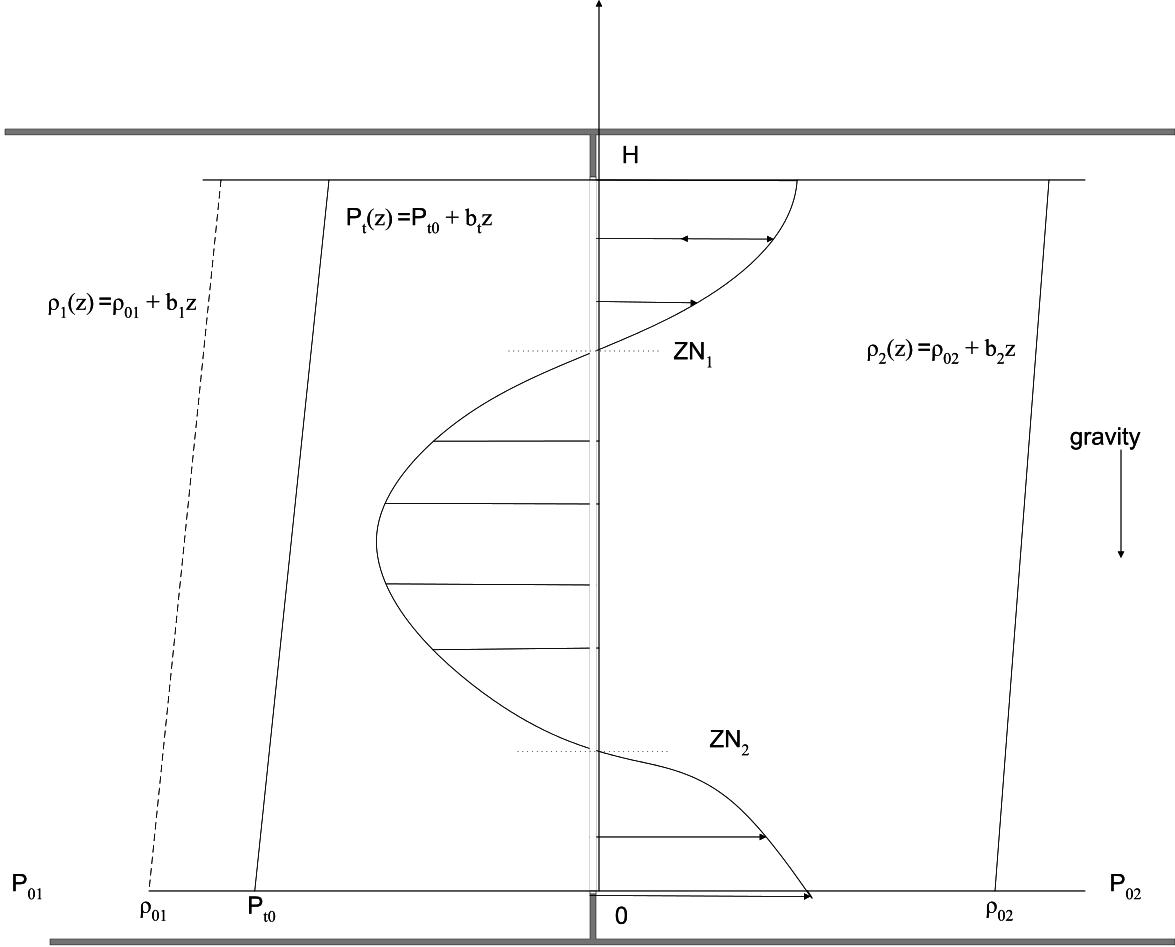
\includegraphics[width=1\linewidth]{img/detailed_opening.png}
		\label{fig:DetailedOpening}
		\begin{flushleft}
			Fonte: \citeonline{EnergyPlus2018}.
		\end{flushleft}
	\end{figure}
	
	O coeficiente de descarga (Cd) é utilizado para representar a característica do fluxo na abertura quando a abertura é grande. Para frestas, utiliza-se o coeficiente de fluxo de ar por frestas \cite{Arendt2017}.
	Esses coeficientes se definem como a razão entre o fluxo real em relação ao	ideal, quando a taxa de fluxo de massa de ar de referência é a vazão mássica de ar para a diferença de pressão de 1 Pa. Ambos os parâmetros dependem da geometria da abertura, velocidade do ar, orientação geográfica, edificações do entorno, morfologia urbana e a forma do edifício em questão.
	O valor do Cd é o produto entre o coeficiente de velocidade e o coeficiente de contração \cite{Flourentzou1998}. Ele pode ser determinado experimentalmente quando a taxa de fluxo de ar é medida diretamente, com gás rastreador, por exemplo. O coeficiente de velocidade também pode ser determinado similarmente medindo-se as velocidades do ar.
	
	\citeonline{Iqbal2015} apontam que o Cd representa os efeitos não ideais de fluxo, que são causados principalmente pela fricção no caminho do fluxo de ar e o efeito de contração devido a mudanças na direção do fluxo. Devido à dificuldade de se estimar esses efeitos separadamente, normalmente apenas o Cd é usado para especificar vazão de ar através de aberturas. O valor de Cd para janelas operáveis não é constante, mas varia consideravelmente de acordo com a área de abertura, o tipo de janela e a diferença de pressão entre a abertura. O uso de valores constantes de Cd podem levar a estimativas errôneas do fluxo de ar.

	De acordo com o manual do COMIS \cite{Feustel1990}, os valores de Cd podem variar de 0,61, para orifícios de arestas vivas,	até 0,98 para tubos com forma de trompete. Os valores encontrados podem variar de 0,25 até 0,75 para grandes aberturas. Normalmente assume-se o valor de 0,6 para aberturas retangulares em simulações  \cite{Flourentzou1998, Heiselberg2001, Breesch2010, Iqbal2015, Krzaczek2015, Arendt2017}.
	
	O objetivo de \citeonline{Flourentzou1998} foi identificar os valores de coeficientes de resistência de fluxo para uma edificação de escritórios de três pavimentos naturalmente ventilada na Suíça. A ventilação por força do vento foi desconsiderada devido à sua instabilidade, o que fez com que os experimentos fossem conduzidos em noites sem vento. O estudo considerou apenas ventilação por força de empuxo, de fluxo levemente turbulento, buscando validar algoritmos simples de ventilação e dar uma base experimental para diretrizes de projeto para técnicas de resfriamento noturno. Nos experimentos, mediu-se a velocidade do ar e linha de pressão neutra, observando-se os coeficientes de contração e de velocidade usados no modelo de Bernoulli. As medições foram efetuadas levando-se em conta a ventilação unilateral e cruzada. As escadas funcionaram como uma chaminé de exaustão nas trocas de ar por empuxo. Os valores de Cd encontrados estão de acordo com o valor geralmente aceito de 0,6 ${\pm}$ 0,1.

	\citeonline{Heiselberg2001} descreveram e sumarizaram os resultados de uma série de medições em laboratório, desenvolvidas para determinar as características do fluxo de ar em janelas abertas, e da distribuição de ar na sala, além de fornecer dados para projetos. O trabalho focou na estimativa dos Cd, nas condições de fluxo de ar no ambiente e no desenvolvimento de um modelo semi-empírico de fluxo para estimar parâmetros de conforto em zonas ocupadas. As medições foram aplicadas a dois tipos de janelas, e em função do ângulo de abertura e diferenças de pressão e temperatura através da abertura. Os resultados mostram que o Cd não pode ser considerado constante, pois varia consideravelmente em função da área de abertura, do tipo de janela e das diferenças de temperaturas. Isso pode levar a erros relacionados à capacidade de fluxo. O valor normalmente adotado de 0,6 é obtido apenas para áreas de abertura grandes. Áreas de abertura menores possuem valores maiores.

	O estudo de \citeonline{Iqbal2015} avalia o efeito do ângulo de abertura na taxa de fluxo ar em janelas pivotantes em telhados. Os valores de Cd são obtidos para os diferentes ângulos, com e sem vento, para fluxos de entrada e saída. Utilizou-se medições em túnel de vento para o estudo, com o modelo de uma residência em escala 1:20. Os resultados são apresentados para fluxo unidirecional. Na ausência de vento, o Cd diminui com o aumento do ângulo de abertura. O Cd mostrou-se variar em função do número de Reynolds. Para fluxo turbulento totalmente desenvolvido, o Cd também diminui com o aumento no ângulo de abertura. Para fluxos de ar movidos por vento, o Cd da janela depende da turbulência na taxa de fluxo de ar que passa pela abertura. Concluiu-se que o valor de Cd varia em função da fração de velocidade (velocidade média do ar em relação à velocidade do vento de referência). Os valores de Cd para fluxos de entrada e saída foram diferentes. Quando a velocidade do ar é superior à velocidade do vento de referência, o Cd é independente da fração de velocidade e da direção do fluxo, e os valores de Cd são idênticos aos valores para velocidade do vento igual a zero. Para ângulos de abertura pequenos o Cd era próximo a 1, enquanto o valor mínimo de Cd foi igual a 0,6 para abertura máxima, valor geralmente utilizado nos modelos de AFN para grandes aberturas. Concluiu-se que janelas pivotantes podem auxiliar na obtenção de valores maiores para o Cd, que varia em relação ao ângulo de abertura.
	
	O fluxo de ar por aberturas horizontais no programa EnergyPlus 8.9 \cite{EnergyPlus2018} é baseado no trabalho de \citeonline{Cooper1989}. Considera-se fluxo de ar por diferença de pressão entre as zonas, por diferença de densidade (causada pelas diferenças de temperatura), ou ambos os fenômenos simultaneamente. A troca de ar total entre as zonas é a soma do fluxo gerado pela diferença de pressão, mais o fluxo da força de empuxo. Porém, o fluxo de ar que desce pela força de empuxo é igual ao fluxo de ar que sobe, cancelando a parcela da força de empuxo no somatório da massa de ar que entra e sai da zona. Para a modelagem de uma escada, há a possibilidade de se considerar um plano inclinado na abertura horizontal. Essa consideração é realizada pela substituição da área de abertura por uma área de abertura efetiva.
	
	A VN é um fenômeno complexo, dependente de diversos fatores. O uso de modelos AFN tem algumas limitações, assim como os coeficientes adotados para a aplicação dos modelos. Apesar das condições de contorno e simplificações adotadas, o AFN apresenta-se como uma solução mais compatível com programas de simulação termoenergética de edificações como o EnergyPlus, devido ao relativo baixo custo computacional e à integração já	existente aos demais algoritmos do programa.
	
	\section{Conforto Térmico}
	
	Dentro de uma edificação, diversos fatores podem influenciar no conforto dos ocupantes, como características acústicas, visuais ou térmicas. Devido ao foco deste trabalho, serão discutidas questões relacionadas ao conforto térmico.
	A busca por conforto térmico tem influência significativa na construção de edificações e na escolha dos materiais construtivos. Esse conforto depende de fatores físicos, fisiológicos e psicológicos. De acordo com a \citeonline{ASHRAEStandard552017}, conforto térmico é o estado da mente que expressa satisfação da pessoa com o ambiente térmico que a circunda, e é estimado através de avaliação subjetiva. No estudo do conforto térmico há duas abordagens principais: o modelo estático e o modelo adaptativo. % \textit{Standard 55}
	O modelo estático foi desenvolvido por \citeonline{Fanger1970a}, a partir de estudos realizados em câmaras climatizadas. As câmaras climatizadas tinham temperatura, umidade relativa e velocidade do ar controladas, e os objetos de estudo exerciam atividades e utilizavam vestimentas específicas. Neste estudo, as variáveis mais importantes que influenciam no conforto térmico são: nível de atividade; resistência térmica das roupas; temperatura do ar; temperatura radiante média; velocidade do ar; umidade relativa no ambiente.

	Para determinar o nível de conforto térmico no ambiente construído, \citeonline{Fanger1970a} desenvolveu a partir dessas variáveis o “Voto Médio Predito” (PMV), uma escala para otimizar as condições de conforto térmico em um ambiente construído. A escala do PMV prediz se os ocupantes do ambiente estarão sentindo frio, calor ou neutros. Para que haja conforto térmico, é necessário que haja neutralidade térmica. A neutralidade térmica é a condição na qual a pessoa prefere que o ambiente à sua volta não esteja nem mais frio, nem mais quente.
	A abordagem no modelo adaptativo é diferente da proposta no modelo estático. De \citeonline{Dear1997} afirmam que uma premissa importante do modelo adaptativo é que o ocupante da edificação não é simplesmente um receptor passivo de um dado ambiente térmico, como no caso das câmaras climáticas, mas em vez disso é um agente ativo, que interage em diversos níveis do sistema “pessoa-ambiente” via ciclos retroalimentados. As expectativas térmicas resultam da confluência de experiências correntes e passadas e práticas técnicas e culturais. Sendo assim, leva-se em conta diferenças não apenas quantitativas, mas também qualitativas entre o conforto térmico em edificações condicionadas artificialmente e naturalmente ventiladas. Baseando-se em um estudo de um banco de dados de 21 mil medições realizadas em edificações comerciais, \citeonline{Dear1997} concluíram que, em edificações ventiladas naturalmente, a tolerância dos usuários em relação à variação de temperatura é maior, e o conforto depende diretamente das temperaturas médias externas.
	
	A relação estabelecida, define os limites inferior e superior de temperatura operativa do ambiente, a partir da temperatura externa média, e estão de acordo com as Equação \ref{eq:limInf} e Equação \ref{eq:limSup} \cite{ASHRAEStandard552017}.
	
	%	\vspace{-8pt}
	\begin{equation}\label{eq:limInf}
	T_{inf} = 14,3 - 0,31 T_m
	\end{equation}
	%	\vspace{-5pt}
	%	\vspace{-8pt}
	\begin{equation}\label{eq:limSup}
	T_{sup} = 21,3 - 0,31 T_m
	\end{equation}
	%	\vspace{-5pt}`
	
	Onde:
	
	$T_{inf}$ é o limite inferior da temperatura operativa para que haja conforto térmico ($^{\circ}$C);
	
	$T_{sup}$ é o limite superior da temperatura operativa para que haja conforto térmico ($^{\circ}$C);
	
	$T_m$ é a temperatura média do ar externo ($^{\circ}$C).
	\\
	
	A temperatura média do ar externo representa o ambiente climático externo com o qual os ocupantes da edificação estão fisiologicamente,
	comportamentalmente e psicologicamente adaptados. Essa variável de entrada é baseada na média aritmética das temperaturas médias externas diárias em um período de dias, e pode ser considerada como a temperatura média mensal.
	
	O movimento do ar influencia no conforto térmico, causando desconforto por frio em algumas situações, mas também aliviando o desconforto por calor.
	Isso ocorre devido ao aumento da convecção sobre as superfícies, o que causa maior evaporação, fenômeno endotérmico. Devido a essa influência no conforto térmico, a \citeonline{ASHRAEStandard552017} permite considerar a velocidade do ar como um fator determinante na busca por um ambiente termicamente confortável. Essa consideração é baseada nos valores do  \textit{Standard Effective Temperature} (SET), que relaciona a velocidade do ar e a temperatura operativa do ambiente para ambientes climatizados.
	
	\citeonline{DeVecchi2015} aplicaram o método adaptativo da \citeonline{ASHRAEStandard552013} para o contexto climático brasileiro, caracterizado como quente e úmido. Os resultados indicam que é possível encontrar níveis aceitabilidade térmica significativos abaixo dos limites inferiores do método adaptativo. Essa tolerância a temperaturas mais baixas deve-se ao aumento de vestimentas por parte dos ocupantes, antes de se recorrer ao aquecimento artificial. Os autores sugerem que a fixação do limite inferior de temperatura operativa em no máximo 19,5 $^{\circ}$C, para umidade relativa de oitenta por cento, representaria mais adequadamente o comportamento dos usuários no contexto climático brasileiro.
	
	\section{Ventilação natural em edifícios de escritórios}
	
	Nesta parte da revisão, buscou-se identificar estudos sobre o uso da VN em edificações de escritórios. Foram identificadas as características dos edifícios relacionadas à geometria, envoltória, padrões de uso, ganhos internos, configuração das aberturas da fachada, entre outros.
	
	Ao longo da maior parte da história, as edificações eram projetadas de forma que o potencial da VN fosse explorado ao máximo. Com a invenção do ar condicionado, a partir da segunda metade do século 20, houve um crescimento do uso de ventilação mecânica e condicionamento de ar no mundo e, com isso, a arquitetura das edificações comerciais começou a sofrer mudanças \cite{CarrilhodaGraca2016} Associado a essa mudança do desenho vernacular tradicional, o desenvolvimento urbano resultou em problemas particulares relacionados à demanda de resfriamento nos meses mais quentes. Os grandes centros urbanos são considerados como uma ilha de poluição. Em muitas cidades, o ambiente externo é contaminado com ruído sonoro, partículas finas, calor e gases tóxicos. A dificuldade na aplicação da VN em edifícios comerciais atualmente se deve ainda a aspectos como a necessidade da concepção do conceito desde as fases iniciais de projeto, ou até mesmo a questões estéticas.
	
	A intensidade de ocupação em edifícios de escritórios varia de acordo com as atividades exercidas. Alguns escritórios são continuamente ocupados por computadores e equipamentos ligados constantemente, enquanto outros são pouco ocupados e têm pouco uso de computadores e iluminação \cite{Elharidi2018}.
	
	\citeonline{Neves2019} desenvolveram um banco de dados com informações levantadas em edifícios de escritórios que operam com ventilação híbrida (VN e condicionamento artificial de ar). Para isso, 153 edifícios construídos após o ano de 1995 na cidade de São Paulo foram selecionados. Dentre os edifícios selecionados, foi realizado um levantamento de campo em 50 edifícios, obtendo-se informações relacionadas às dimensões das salas de escritórios, ao tipo de esquadria utilizado e à presença de elementos de sombreamento. As informações disponíveis em todos os edifícios do banco de dados incluem: áreas, dimensões, formato e número de pavimentos das edificações; absortância das paredes externas e coberturas; e percentual de abertura na fachada (PAF). Os autores observaram as correlações entre as características encontradas nestes edifícios. As estratégias de VN adotadas não parecem ser algo que procura-se otimizar nos projetos dos edifícios analisados. Tampouco há indicação de uma mudança nesse cenário em edificações de anos mais recentes. O que se nota é o aumento de elementos de sombreamento na fachada em razão do uso de equipamentos condicionadores de ar do tipo split. Os autores concluem que o levantamento realizado permite a identificação das características mais recorrentes nos edifícios analisados, e os intervalos de variação nos parâmetros observados.
	Isso possibilita que trabalhos relacionados ao desempenho térmico de edificações sejam desenvolvidos considerando-se características de edificações reais.
	
	\citeonline{Belleri2014} compararam predições de desempenho de VN em estágio inicial de projeto pelo programa EnergyPlus com medições de campo. O escritório estudado localiza-se no segundo andar de um edifício de dois andares na Califórnia, Estados Unidos, e tem seu espaço dividido em dois planos abertos de 130 m2, conectados por duas grandes aberturas. Não há ventilação forçada ou sistema de resfriamento. As quatro fachadas são providas de janelas, que podem ser operadas pelos ocupantes. Há ventiladores de teto com controle variável disponíveis. Os autores partiram da simulação de um modelo simples, e modificaram gradativamente os seguintes dados de entrada, de acordo com medições em campo: temperaturas internas; controle das janelas; dados climáticos (com intervalos de 5 minutos); fatores de abertura das janelas, coeficientes de pressão do vento (baseados em medições em túnel de vento). Enquanto a simulação inicial superestimou a média das trocas de ar em 1671\%, a simulação com todas as modificações superestimou as trocas de ar em apenas 148\%. O estudo conclui que, com dados suficientes, a utilização do programa EnergyPlus com o AFN pode oferecer  estimativas informativas relacionadas ao desempenho da VN. No entanto, para melhores estimativas é necessário obter dados relacionados ao vento e ao comportamento dos ocupantes, o que pode ser dificultoso na fase de projeto.

	O trabalho realizado por \citeonline{Elharidi2018} buscou identificar o desempenho energético e a qualidade do ar interno de edifícios de escritórios no Egito, propondo medidas para minimizar o uso de energia. Os dados foram levantados a partir de questionários realizados em 59 escritórios, sendo complementado por dados da literatura. Os dados registrados incluem: área interna, atividade exercida no escritório, tipo de serviço prestado na edificação, tipo de edificação, e contas de energia elétrica. Dentre as atividades nos escritórios, inclui-se contadores, agências de viagem, vendas, administração da saúde, seguros, consultores, administração de bancos, recursos humanos, e governo. As edificações de escritórios foram classificadas em quatro tipos: VN sem resfriamento; VN com resfriamento local; ventilação mecânica com resfriamento local; ventilação mecânica e resfriamento central. A maioria das edificações estudadas possui apenas ventilação natural, ou VN com resfriamento local. A estratégia adotada para resfriamento e ventilação dos edifícios foi identificada como o fator mais impactante no consumo de energia. A eficiência dos equipamentos, iluminação e sistemas de resfriamento, relacionada ao comportamento dos ocupantes, pode reduzir significativamente o consumo elétrico da edificação. 
	Os edifícios com apenas VN têm os menores consumos de energia, sendo que há a possibilidade de desconforto térmico em certas épocas do ano sob essas condições. Os edifícios com VN e resfriamento local têm maior consumo de energia nos meses de verão, mas demandam menos da metade do consumo de energia dos edifícios com resfriamento central.
	
	O estudo de \citeonline{Roetzel2014} investigou o impacto do projeto da edificação e da ocupação no conforto térmico e desempenho energético em escritórios, para identificar padrões que ajudem nas considerações relacionadas aos estágios iniciais de projeto. O estudo baseia-se no cenário A2 do \textit{International Panel on Climate Change} (IPCC), para o ano de 2030.
	Uma sala de escritório celular foi modelada e simulada para três climas através do programa EnergyPlus. Os locais considerados são: Hamburgo, Alemanha; Atenas, Grécia; e Alice Springs, Austrália. Dentre as variações no projeto, considerou-se três tipos de construções: de luxo; de baixo custo inicial; e sustentável. As considerações relacionadas ao comportamento dos ocupantes foram duas: de pior cenário; e de cenário ideal. Para avaliar o conforto térmico e o desempenho energético, as simulações foram realizadas para duas condições: sem consideração de resfriamento e aquecimento para análise de conforto; e incluindo-se \textit{setpoints} para aquecimento e resfriamento.
	O estudo conclui que os comportamento dos ocupantes é o que mais influencia no consumo final de energia para todos os climas investigados.
	Para buscar um melhor desempenho e melhores níveis de conforto, as seguintes estratégias para o projeto da edificação são indicadas: proteção solar externa que permita iluminação natural; PAF maiores que 70\% e janelas localizadas acima do plano de trabalho; massa térmica aplicada ao piso, paredes e cobertura. Em relação ao comportamento dos ocupantes, as estratégias sugeridas são: operar ativamente as janelas durante o dia e também para a ventilação noturna; operar venezianas para aproveitar a iluminação natural, prevenindo-se de ofuscamento e calor; operar iluminação artificial dependendo da luz natural; e utilizar equipamentos de escritório com baixa potência de consumo.
	
	\citeonline{Pesic2018} descrevem a aplicabilidade geoclimática da VN na região da Catalunha, na costa do Mediterrâneo. O objetivo é providenciar diretrizes e parâmetros básicos de eficiência energética para arquitetos, engenheiros e políticos, para que possam visualizar o potencial da VN. Três cidades foram analisadas: Barcelona; Terrassa; e Tarragona. O modelo de escritório representa um edifício de três pavimentos \textit{open-plan}. A ventilação cruzada é modelada considerando-se a passagem de ar por janelas operáveis, com movimento gerado primariamente por força do vento. A orientação da edificação foi definida perpendicularmente à principal direção do vento nos meses em que a VN é mais favorável. O PAF é definido como 40\% e a infiltração na envoltória é considerada constante, com 0,25 trocas de ar por hora. As temperaturas limite de aceitabilidade do ar externo para VN é entre 10 $^{\circ}$C e 33,5 $^{\circ}$C. O horário de ocupação é das 8h00 às 18h00, e a ventilação noturna é das 21h00 às 7h00. Considerou-se a possibilidade de uso de condicionamento de ar para aquecimento e resfriamento, ou ventilação mecânica (HVAC) entre as 6h00 e 18h00. A ocupação foi considerada apenas nos dias de semana. A construção e isolamento da edificação foram definidos de acordo com os padrões da Passivhaus, padrão de construção baseado no uso de isolamento térmico da edificação. A VN foi considerada entre os dias 1º de abril e 31 de outubro (meses quentes). Seis modos de resfriamento foram considerados na análise: apenas HVAC; VN ou HVAC; VN ou HVAC, e ventilação noturna; VN e HVAC simultaneamente; VN e HVAC simultaneamente, e ventilação noturna; apenas ventilação noturna. O maior potencial de redução de energia foi observado para o uso simultâneo de HVAC e VN, com ventilação noturna. Em relação ao caso com apenas HVAC, a redução relativa foi de 28,4\%, em Tarragona, a 40,9\%, em Barcelona.
	
	O estudo de \citeonline{Yao2009} buscou um método de analisar estrategicamente o uso de VN nas etapas iniciais de projeto. Consideraram-se as condições climáticas locais, tipo de edificação, padrões de ocupação e ventilação. O trabalho é desenvolvido a partir de um modelo de escritório para cinco climas da China: muito frio; frio; verão quente e inverno frio; verão quente e inverno ameno; e ameno. Os escritórios na China se dividem em dois tipos principais: de alto padrão com sistema central de ar condicionado; e escritório tradicional com ar condicionado \textit{split}. O modelo de escritório utilizado para o estudo possui as seguintes características: sala com dimensões 3,6 m x 5,4 m x 3,0 m; orientação sul-norte; PAF de 0,35 na parede sul e 0,25 na parede norte; ocupação das 8h00 às 18h00; capacidade térmica média; elementos de sombreamento interno na fachada sul no verão; tipo de terreno urbano; ganhos internos igual a 25 W/m2. Os autores concluem que em zonas de clima ameno a VN é altamente recomendável para edifícios de escritório em ambos os turnos. A ventilação cruzada tem maior eficiência do que a ventilação unilateral.
	Em zonas de verão quente e inverno ameno, o uso de VN não satisfaz as exigências para conforto térmico. Portanto, o resfriamento mecânico é recomendado. Observou-se que o uso unicamente da ventilação noturna a não é adequada para edifícios de escritórios, pois os ganhos internos gerados ao longo do dia não podem ser liberados, causando desconforto térmico. 
	
	\citeonline{Yun2008} comentam a dificuldade de se modelar o comportamento dos ocupantes, e como esse aspecto é uma barreira na exploração do uso de técnicas passivas e mistas de eficiência energética. Um estudo de caso foi conduzido durante o verão em seis salas de escritório com VN, localizados em Cambridge, Reino Unido. Os escritórios são ocupados por uma ou duas pessoas, e têm o PAF variando entre 0,12 e 0,57. Dentre os objetivos do estudo, buscou-se examinar o potencial da VN como estratégia de conforto e resfriamento. Foram coletados dados relacionados à posição das janelas e temperaturas internas e externas, além da aplicação de questionários.
	Dos casos analisados, o que obteve melhor índice de conforto foi o escritório com brise externo e com possibilidade de aplicação de ventilação noturna. O caso com maior desconforto por calor possui uma janela com PAF de 0,57 orientada para oeste, sem sombreamento externo. As análises mostram que elementos do projeto como a orientação da fachada, o tamanho da janela em relação à orientação, a possibilidade de ventilação natural pela janela, e o sombreamento externo por brise ou edificações vizinhas são fatores determinantes no desempenho térmico. Os autores apontam que áreas envidraçadas menores podem melhorar o desempenho térmico, mas podem comprometer o uso da iluminação natural. Portanto, é crucial buscar um equilíbrio entre o uso de iluminação natural e a busca por minimizar os ganhos de calor pela fachada. Os resultados sugerem que a VN como um método de resfriamento passivo nem sempre é efetiva, pois os ocupantes nem sempre operam as janelas de acordo com as condições ideais para o resfriamento por ventilação. Portanto, destaca-se a importância de se elaborar um projeto robusto para a edificação, para compensar comportamentos desfavoráveis por parte dos ocupantes.

	De acordo com \citeonline{CarrilhodaGraca2016}, nos climas quentes, que é o caso do Brasil, há maior potencial de economia e maior desafio na aplicação de VN. \citeonline{Roetzel2014} afirmam que o modelo adaptativo da \citeonline{ASHRAEStandard552017} tem uma faixa maior de aplicabilidade em climas mais quentes, o que pode propiciar um maior potencial de otimização.
	Esta parte da revisão bibliográfica apresentou estudos que abordam o potencial de VN como uma solução para o resfriamento passivo em edificações de escritórios. Nos diferentes casos e configurações dos sistemas de resfriamento considerados, algumas características avaliadas e soluções propostas são predominantes, como o uso de ventilação cruzada ou de sombreamento das aberturas.
	No entanto, a variação de determinadas características das edificações podem resultar em desempenhos térmicos diferentes de acordo com as combinações de parâmetros, ou características climáticas 
	
	\section{Análise de sensibilidade}
	
	Análise de sensibilidade (AS) é uma ferramenta valiosa na simulação termoenergética de edificações. Por isso, a AS é usada amplamente para explorar as características do desempenho térmico em edificações em diversas aplicações, como projetos, calibração de modelos, \textit{retrofits}, impacto das mudanças climáticas entre outros \cite{Tian2013a}. A metodologia para a aplicação da AS tipicamente adota os seguintes passos: determinar as variações dos dados de entrada; determinar os modelos das edificações; executar as simulações dos modelos; coletar os resultados; executar a AS; apresentar os resultados da AS. Os métodos de AS podem ser divididos entre as abordagens local e global. A AS local é focada nos efeitos da incerteza de parâmetros de entrada em torno de um caso base, enquanto a AS global é mais interessada na influência dos parâmetros de entrada sobre todo o espaço de parâmetros de entrada possíveis. Por isso, a AS global é considerada mais confiável. A AS global inclui métodos de regressão, baseados em screening, em variância e metamodelos.
	
	O primeiro passo para realizar uma AS é determinar a faixa dos dados de entrada. Quando o objetivo é determinar diferentes opções de projeto,  \citeonline{Tian2013a} sugere distribuições uniformes nos dados de entrada, pois assume-se que os diferentes valores para os dados de entrada são igualmente prováveis.
	
	O método da variância decompõe a incerteza dos dados de saída para seus correspondentes dados de entrada  \cite{Tian2013a}. Nessa abordagem, os dois métodos mais comuns são o FAST \cite{Saltelli2004} e o \citeonline{Sobol1993}. 
	Por esses métodos, é possível avaliar efeitos de primeira ordem e de ordens superiores.
	Os efeitos de primeira ordem são determinados observando-se o quanto a variação de cada parâmetro isoladamente influencia na variância dos dados de saída.
	Os efeitos de segunda ordem consideram as interações entre dois parâmetros na variância dos dados de saída, e a mesma lógica segue para os efeitos de ordens superiores.
	Os efeitos totais, para cada parâmetro, são a soma dos efeitos de todas as ordens.
	Ao somar os efeitos de primeira ordem mais os efeitos de ordens superiores, de todos os parâmetros do modelo, o valor obtido deve ser igual a 1.
	Quando o objetivo é fixar parâmetros não importantes, os efeitos totais devem ser usados \cite{Saltelli2004}. Métodos de variância são de abordagem livre, fazendo com que sejam adequados para modelos não-lineares e com correlações entre variáveis.
	
	\section{Metamodelos de eficiência energética e desempenho térmico em edificações}
	Projetistas encontram dificuldades no uso de ferramentas de simulação de desempenho energético, que podem não ser compatíveis com suas necessidades e métodos de trabalho. Por isso, \citeonline{Picco2014a} propõem simplificar a descrição do edifício e converter um modelo detalhado em um modelo simplificado, com apenas um número limitado de entradas. Em um estudo de caso, simplificações foram assumidas quanto às envoltórias, superfícies transparentes, zonas térmicas e pavimentos de um edifício comercial. As diferenças encontradas em relação ao modelo detalhado, no pior caso, foram de 15,6\% para cargas de aquecimento e 14,6\% para cargas de resfriamento. Com diferenças menores de 4\% e 9\% para cargas de pico, respectivamente. Apesar das margens de erro, os autores observaram que simplificações no modelo podem auxiliar em estágios iniciais de projeto, quando certas características no projeto do edifício ainda não estão bem definidas.
	
	Há modelos baseados em equações físicas, que simulam os sistemas de transferência de calor, e modelos baseados em funções estatísticas, que deduzem esses comportamentos. Modelos estatísticos funcionam apenas com entradas e saídas, sem correlacionar causa e efeito, mas têm maior agilidade. 
	Os modelos escritos com equações físicas seguem os princípios da conservação de energia e são os que mais se aproximam do comportamento real, mas podem ser dificultosos de se aplicar por serem muito complexos. Para adaptar as principais funcionalidades de ambos os modelos, existem modelos híbridos, chamados metamodelos.
	
	Modelos preditivos são funções matemáticas que, aplicadas a uma quantidade significativa de dados, conseguem identificar padrões ocultos e prever o que poderá ocorrer. Os métodos de inteligência artificial mais utilizados para predição d`e desempenho energético de edificações são redes neurais artificiais (RNA) e máquinas de vetores de suporte (MVS) \cite{Zhao2012}. São modelos altamente eficazes na solução de problemas não-lineares. Esses métodos podem oferecer predições altamente precisas, desde que as definições do modelo e parâmetros estabelecidos estejam definidos adequadamente. Modelos de RNA já foram usados para analisar vários tipos de consumo de energia em edificações em diversas condições, como em cargas de aquecimento e resfriamento, consumo de eletricidade, operação e otimização de componentes, e estimativa de parâmetros de uso. O uso de MVS vem crescendo em pesquisas e indústria. Em muitos casos as MVS mostram performances superiores às das RNA, mesmo com pequena quantidade de dados para treinamento.
	
	Os resultados de simulações podem ser avaliados a partir de características específicas. Essas características podem incluir pico da demanda de energia, consumo anual de energia, conforto, custo do ciclo de vida, entre outros. No desenvolvimento de um metamodelo analítico para otimização de modelos de energia de edificações, \citeonline{Eisenhower2012} utilizaram o PMV para a avaliação dos resultados. A caracterização dos dados e técnica de regressão do modelo foram baseadas em princípios de aprendizagem automática. Aprendizagem automática é uma classificação de algoritmos que tentam identificar características dentre os dados, sem conhecimento prévio dessas características. 
	Dentre diferentes possíveis abordagens (RNA, Programação Genética, Redes Bayesianas) a escolhida para o caso foi a MVS. 
	A identificação dos parâmetros mais influentes no processo de otimização foi realizada através de uma análise de sensibilidade global, baseada em derivadas locais. O metamodelo gerado foi capaz de identificar a minimização do consumo de energia, mantendo ou melhorando o conforto, sem necessidade de extensivas repetições de simulações de energia.
	
	\citeonline{Rackes2016} propõem um metamodelo para analisar edificações comerciais e escolas de poucos pavimentos, ventiladas naturalmente. Primeiramente, foi construído um banco de dados com aproximadamente 50.000 simulações. As simulações foram executadas a partir dos modelos termoenergéticos e AFN do programa EnergyPlus, e do modelo de conforto adaptativo da  \citeonline{ASHRAEStandard552013}, que determina a zona de conforto que satisfaz 80\% dos ocupantes. As características dos edifícios simulados foram variadas a partir de 55 dados de entrada relacionados à tipologia do edifício, layout interno, geometria das janelas e sombreamento, propriedades do fluxo de ar, materiais de construção, cargas internas e transferência de calor pelo solo. Os arquivos de IDF utilizados pelo EnergyPlus foram criados a partir de uma rotina escrita no programa MatLab. Foram utilizados 427 arquivos climáticos do Brasil para a representação geográfica. 
	O indicador de desempenho em conforto térmico escolhido foi o \textit{Exceedance Hour Fraction} (EHF), que é a fração de horas de desconforto em relação às horas de ocupação. Na etapa seguinte, 93 parâmetros preditores foram definidos para a análise do banco de dados. A principal ferramenta para a análise de sensibilidade foi a regressão linear múltipla da variável resposta em relação aos preditores. O método de aprendizagem automática escolhido foi a MVS. Após treinar e avaliar diversos modelos, 53 parâmetros preditores foram selecionados para a versão final. Esses parâmetros podem ser obtidos a partir de 29 dados de entrada e um arquivo climático. Comparando as simulações do EnergyPlus com as predições, o metamodelo apresentou RMSE (erro médio quadrático) igual a 0,059 e AE95 (erro absoluto do 95o percentil) igual a 0,126. Quando testado com outros 2000 casos não usados no treinamento do metamodelo, o RMSE foi 0,060 e o AE95 foi 0,129, o que indica consistência nos resultados. 
	
	\citeonline{Versage2015} desenvolveu um metamodelo para estimar a carga integrada anual de energia de refrigeração para avaliação de desempenho energético de edificações condicionadas artificialmente através do desempenho individual de suas zonas térmicas. Foi desenvolvida uma base de dados de aproximadamente 1,29 milhões de casos simulados, com parâmetros construtivos variados, para o clima de Florianópolis. Uma amostra dos dados foi adotada para a elaboração de metamodelos com as técnicas de regressão linear múltipla, regressão adaptativa multivariada por \textit{splines}, processo gaussiano, máquina de vetores de suporte, \textit{random forest} e redes neurais artificiais. Para avaliar e comparar os metamodelos, quatro índices de desempenho foram escolhidos: tempo de treinamento, coeficiente de determinação (R$^2$), RMSE e erro médio quadrático normalizado (NRMSE). O metamodelo de RNA obteve o melhor desempenho entre os testados. A rede neural artificial treinada com 1\% dos casos do banco de dados, e com 72 nós na camada interna, obteve o melhor desempenho global, e foi capaz de reproduzir resultados com erros menores que 10\% para 99,2\% do casos. O metamodelo elaborado a partir de MVS obteve o pior desempenho. Porém, o autor destaca que outras configurações e tratamentos dos dados poderiam mudar o desempenho dos metamodelos avaliados.

%\bibliographystyle{lib/abntex2-num}
%\bibliographystyle{lib/abntex2-alf}
%\bibliography{citacoes}
\bibliography{library}
	
\end{document}